\section{A Probabilistic Model of Feature Selection}

Feature selection is the selection of a subset of features $F^*$ from the complete feature space $F,$ for a specific classification/prediction problem, without loosing too much performance on some given measures. The benefit of feature selection include more explainable model, reduced computation time/power, and the avoidance of overfitting.

Existing feature selection algorithms, whose performance show no statistical difference on out benchmark, are mostly ad-hoc. They give various answers to optimisation, but none of them gives the question. In this project, we started from the first principles, proposed a graphical model, and built a new feature selection system upon it.

\subsection{Graphical Model}

To begin the derivation, we propose a graphical model of feature selection for binary classification problem, as shown in figure~\ref{fig:model}. Double-circle nodes represent observed variables, including the data point vector $\vec{x}^{\,d},$ selected features $f_i^*$ (where $1\leq i\leq k,$ $f_i\in F$) and the supervised class label $y^d.$ Single-circle nodes represent latent variables, including a selected attribute of data point vector $f_i^x,$ and prediction from a feature $y^d_i.$ 

Since jointly optimising this objective is NP-hard, we will build $F^*$ in a greedy manner by choosing the next optimal feature $f^*_k$ given the previous set of optimal features $F^*_{k-1}$ and recursively defining $F^*_k = F^*_{k-1}\cup f^*_k$ with $F^*_0 = \emptyset$. The measure of the fitness of a model can either be Expectation or Likelihood.

\begin{figure}[tbp!]
	\centering
	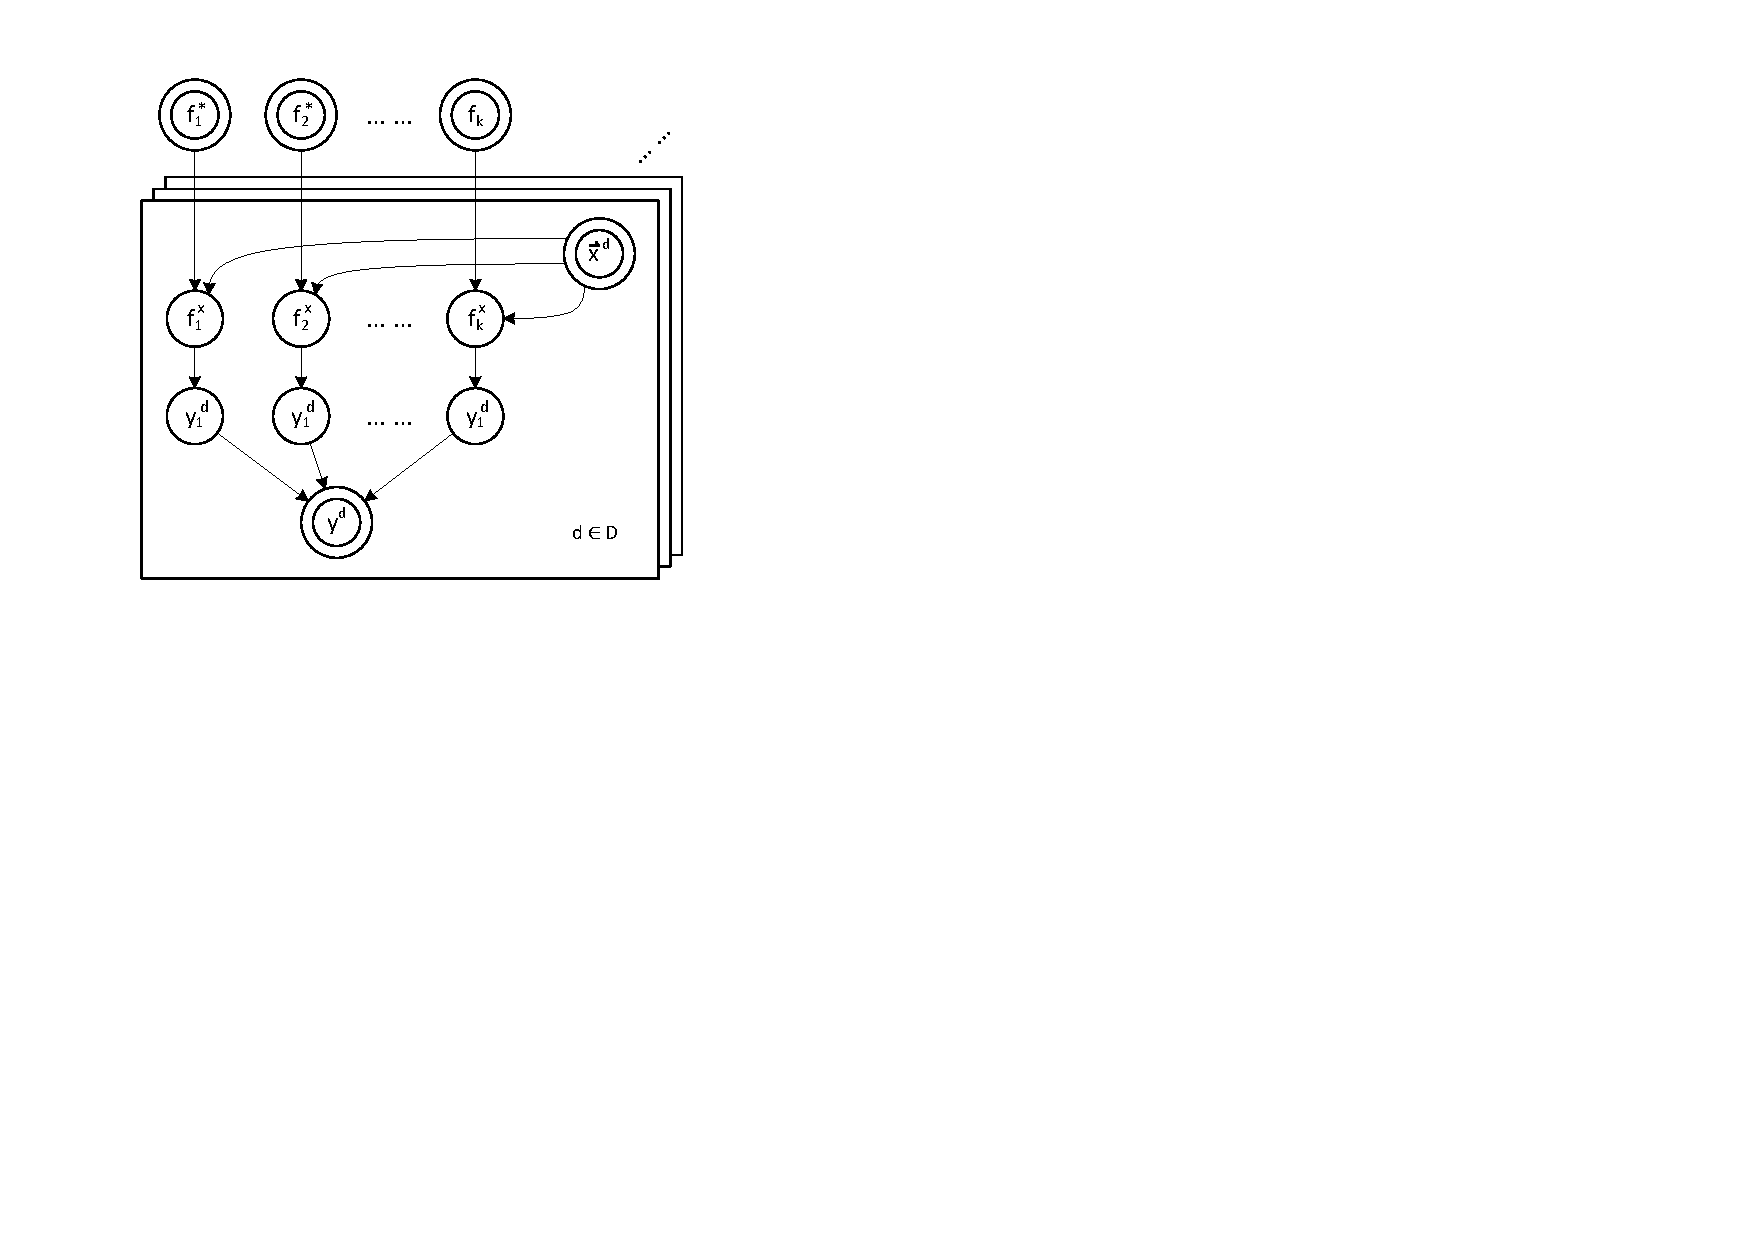
\includegraphics[scale=0.9]{Plots_1.pdf}
	\caption{Graphical model. Double-wall circle denotes observed nodes, single-wall circle denotes hidden nodes.}
	\label{fig:model}
\end{figure}

\section{Expectation}
The initial objective is defined as:
\[f_k^*=\argmax_{f_k}E_D\left[P\left(y^d|\vec{x}^{\,d},F_k\right)\right]\]

\begin{align}
f_k^*&=\argmax_{f_k}E_D\left[P\left(y^d|\vec{x}^{\,d},F_k\right)\right]\nonumber\\
&=\argmax_{f_k}\frac{1}{|D|}\sum_{d\in D} P\left(y^d | \vec{x}^{\,d},F_k\right)\nonumber\\
&=\argmax_{f_k}\sum_{d\in D}\frac{P\left(y^d,\vec{x}^{\,d},F_k\right)}{P\left(\vec{x}^{\,d},F_k\right)}\nonumber\\
&=\argmax_{f_k}\sum_{d\in D}\sum_{\{y_{i}^d\}_{1\leq i\leq k}}\frac{P\left(y^d,\vec{x}^{\,d},F_k,\{y_{i}^d\}_{1\leq i\leq k}\right)}{P\left(\vec{x}^{\,d},F_k\right)}\nonumber\\
=\argmax_{f_k}&\sum_{d \in D}\sum_{{\{y_{i}^d\}}_{1\leq i\leq k}}\frac{P\left(y^d|\{y^d_i\}_{1\leq i\leq k}\right)\left(\prod_{i=1}^kP\left(y_i^d|\vec{x}^{\,d}, f_i\right)\right)P\left(\vec{x}^{\,d}\right)\prod_{i=1}^kP\left(f_i\right)}{P\left(\vec{x}^{\,d},F_k\right)}\nonumber\\
&=\argmax_{f_k}\sum_{d\in D}\sum_{\{y_i^d\}_{1\leq i\leq k}}P\left(y^d|\{y^d_i\}_{1\leq i\leq k}\right)\prod_{i=1}^kP\left(y_i^d|\vec{x}^{\,d},f_i\right)\label{eq:expect}
\end{align}

Here, we rewrote the expectation of a binary event as its probability, factorized the conditional probability in the joint probability divided by the marginal, marginalised over $\{y^d_i\}_{1\leq i\leq k}$, factorized joint probability in conditional and prior following the graphical model and exploited d-separation to remove irrelevant conditions and to cancel terms in the equation.

Now we can optimise our initial objective aiming three goals of classification tasks: Precision, Recall, and General n-out-of-k.

\subsection{Precision}
In order to select the subset of features providing high precision binary classifier we need the agreement of all features predictors $y^d_i$ to predict true. That is, when $y^d$ is true we need all of the predictors $y^d_i$ equals to true, and if $y^d$ were false, just one of the predictors $y^d_i$ would have to be false. Then the probability $P\left(y^d|\{y^d_i\}_{1\leq i\leq k}\right)$ can be expressed as follows:
\begin{equation}
P\left(y^d|\{y^d_i\}_{1\leq i\leq k}\right)=I\left[y^d=\bigwedge_{i=1}^k y^d_i\right]=
\begin{cases}
	y^d=1 \text{ when } \{y_i^d=1\}_{1\leq i\leq k}\\
	y^d=0 \text{ when } \{y_i^d\}_{1\leq i\leq k,\exists{y_j^d\|y_j^d=0}}
\end{cases}\label{eq:expect_pre_1}
\end{equation}
Then, we combined equations \eqref{eq:expect} and \eqref{eq:expect_pre_1}, separated each term according to the actual label value $y^d$ and used the probability sum rule to rewire the second term as follows:
\begin{align}
f_k^*&=\argmax_{f_k}\sum_{d\in D}I\left[y^d=\bigwedge_{i=1}^k y^d_i\right]\prod_{i=1}^kP\left(y_i^d|\vec{x}^{\,d},f_i\right)\nonumber\\[0.5em]
&=\argmax_{f_k}\sum_{d\in D}
\begin{cases}
	y^d=1: \prod_{i=1}^kP\left(y_i^d=1|\vec{x}^{\,d},f_i\right)\\
	y^d=0: \sum_{\substack{\{y_i^d\}_{1\leq i\leq k},\\ \exists{y_i^d\|y_i^d=0}}}\prod_{i=1}^kP\left(y_i^d|\vec{x}^{\,d},f_i\right)
\end{cases}\nonumber\\[0.5em]
&=\argmax_{f_k}\sum_{d\in D}
\begin{cases}
	y^d=1: \prod_{i=1}^kP\left(y_i^d = 1|\vec{x}^{\,d},f_i\right)\\
	y^d=0: 1-\prod_{i=1}^kP\left(y_i^d = 1|\vec{x}^{\,d},f_i\right)
\end{cases}\label{eq:expect_pre_2}\\[0.5em]
&=\argmax_{f_k}\sum_{d\in D}
\begin{cases}
	y^d=1: \prod_{i=1}^kP\left(y^d = 1|\vec{x}_i^{\,d},f_i\right)\\
	y^d=0: 1-\prod_{i=1}^kP\left(y^d = 1|\vec{x}_i^{\,d},f_i\right)\nonumber
\end{cases}
\end{align}
From \eqref{eq:expect_pre_2} we can intuitively describe how this equation is related to the precision metric. In the confusion matrix, Precision is calculated dividing the numbers of true positives by the number of all examples predicted as positive (true positives and false positives). When $y^d$ is true, \eqref{eq:expect_pre_2} gives higher score to feature that have higher probability to predict true, encouraging true positives. Meanwhile, if $y^d$ is false, \eqref{eq:expect_pre_2} gives lower score to features that have higher probability to predict true, penalising false positives.

\subsection{Recall case}
In order to select the subset of features providing high recall binary classifier we need at least one $y^d_i$ to predict true. Therefore, we need a disjunction operation between the predictors $y^d_i$. That is, when $y^d$ is true, we need at least one predictor $y^d_i$ to equals to true, and if $y^d$ were false, all of the predictors $y^d_i$ would have to be false. Then the probability $P\left(y^d|\{y^d_i\}_{1\leq i\leq k}\right)$ can be expressed as follows:
\begin{equation}
P\left(y^d|\{y^d_i\}_{1\leq i\leq k}\right)=I\left[y^d=\bigvee_{i=1}^k y^d_i\right]=
\begin{cases}
	y^d=1 \text{ when } \{y_i^d\}_{1\leq i\leq k,\exists{y_j^d\|y_j^d=1}}\\
	y^d=0 \text{ when } \{y_i^d=0\}_{1\leq i\leq k}
\end{cases}\label{eq:expect_recall_1}
\end{equation}
Here, we combined equations \eqref{eq:expect} and \eqref{eq:expect_recall_1}, separated each term according to the actual label value $y^d$ and used the probability sum rule to rewrite the second term as follows:
\begin{align}
f_k^*&=\argmax_{f_k}\sum_{d\in D}I\left[y^d=\bigvee_{i=1}^k y^d_i\right]\prod_{i=1}^kP\left(y_i^d|\vec{x}^{\,d},f_i\right)\nonumber\\[0.5em]
&=\argmax_{f_k}\sum_{d\in D}
\begin{cases}
	y^d=0: \prod_{i=1}^kP\left(y_i^d=0|\vec{x}^{\,d},f_i\right)\\
	y^d=1: \sum_{\substack{\{y_i^d\}_{1\leq i\leq k},\\ \exists{y_i^d\|y_i^d=1}}}\prod_{i=1}^kP\left(y_i^d|\vec{x}^{\,d},f_i\right)
\end{cases}\nonumber\\[0.5em]
&=\argmax_{f_k}\sum_{d\in D}
\begin{cases}
	y^d=0: \prod_{i=1}^kP\left(y_i^d=0|\vec{x}^{\,d},f_i\right)\\
	y^d=1: 1-\prod_{i=1}^kP\left(y_i^d=0|\vec{x}^{\,d},f_i\right)
\end{cases}\label{eq:expect_recall_2}\\
&=\argmax_{f_k}\sum_{d\in D}
\begin{cases}
	y^d=0: \prod_{i=1}^kP\left(y^d=0|\vec{x}_i^{\,d},f_i\right)\\
	y^d=1: 1-\prod_{i=1}^kP\left(y^d=0|\vec{x}_i^{\,d},f_i\right)
\end{cases}\nonumber
\end{align}
From \eqref{eq:expect_recall_2} we can intuitively describe how this equation is related to the precision metric. In the confusion matrix, Recall is calculated dividing the numbers of actual true positives by the number of all true positives (true positives and false negatives). When $y^d$ is false, \eqref{eq:expect_recall_2} gives higher score to feature that have higher probability to predict false, encouraging true negatives. Meanwhile, if $y^d$ is true, \eqref{eq:expect_recall_2} gives lower score to features that have higher probability to predict false, penalizing false negatives.

\subsection{Likelihood}
\begin{align}
f_k^*&\equiv\argmax_{f_k}\,log\prod_{d\in D}P\left(y^d|\vec{x}^{\,d},F_k\right)\nonumber\\
&=\argmax_{f_k}\sum_{d\in D}log\left(\frac{P\left(y^d,\vec{x}^{\,d},F_k\right)}{P\left(\vec{x}^{\,d},F_k\right)}\right)\nonumber\\
&=\argmax_{f_k}\sum_{d\in D}log\sum_{\{y_i^d\}_{1\leq i\leq k}}\frac{P\left(y^d,\vec{x}^{\,d}, F_k,\{y_i^d\}_{1\leq i\leq k}\right)}{P\left(\vec{x}^{\,d},F_k\right)}\nonumber\\
&=\argmax_{f_k} \sum_{d \in D} log\sum_{{\{y_i^d\}}_{1\leq i \leq k}} \frac{P\left(y^d| \{y^d_i\}_{1 \leq i \leq k}\right) \prod_{i=1}^kP\left(y_i^d|\vec{x}^{\,d},f_i\right)P\left(\vec{x}^{\,d}\right)\prod_{i=1}^kP\left(f_i\right)}{P\left(\vec{x}^{\,d}, F_k\right)}\nonumber\\
&=\argmax_{f_k}\sum_{d\in D}log\sum_{{\{y_i^d\}}_{1\leq i\leq k}}P\left(y^d|\{y^d_i\}_{1\leq i\leq k}\right)\prod_{i=1}^kP\left(y_i^d|\vec{x}^{\,d},f_i\right)\nonumber
\end{align}
Here, we rewrote the likelihood of a binary event as its probability, factorized the conditional probability in the joint probability divided by the marginal, marginalized over $\{y^d_i\}_{1\leq i\leq k}$, factorized joint probability in conditional and prior following the graphical model and exploited d-separation to remove irrelevant conditions and to cancel terms in the equation.

Since $\sum_{d\in D}log\sum_{{\{y_i^d\}}_{1\leq i\leq k}}P\left(y^d|\{y^d_i\}_{1\leq i\leq k}\right)\prod_{i=1}^kP\left(y_i^d|\vec{x}^{\,d},f_i\right)$ is exactly the same as the result in the expectation case, and the logarithm is a monotonous function, the choice of likelihood instead of expectation has no further affect on the algorithm.
